\chapter{总体设计}
\section{软件描述}
系统包括前台和后台两个部分。

前台主要功能是:提供各种功能的查询窗口

后台主要功能是:对各种请求相应

\section{处理流程}
\subsection{总体流程}
此处应当有一个图和对应的描述。

\begin{figure}[H] %H为当前位置,!htb为忽略美学标准,htbp为浮动图形
    \centering %图片居中
    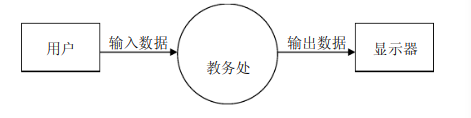
\includegraphics[width=0.7\textwidth]{选区_001} %插入图片,[]中设置图片大小,{}中是图片文件名
    \caption{总体流程} %最终文档中希望显示的图片标题
    \label{Fig.main2} %用于文内引用的标签
\end{figure}

\subsection{客户端基本流程}
\begin{figure}[H] %H为当前位置,!htb为忽略美学标准,htbp为浮动图形
    \centering %图片居中
    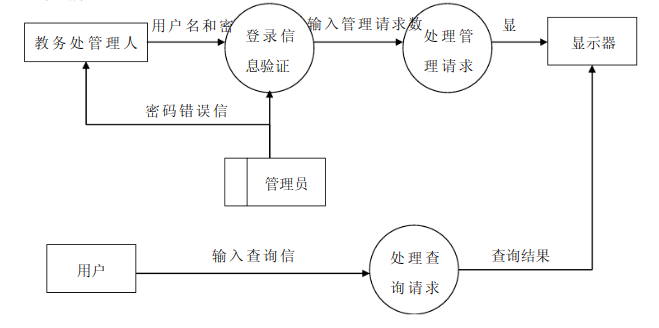
\includegraphics[width=0.7\textwidth]{选区_002} %插入图片,[]中设置图片大小,{}中是图片文件名
    \caption{客户端基本流程} %最终文档中希望显示的图片标题
    \label{Fig.main2} %用于文内引用的标签
\end{figure}

\subsection{服务器端基本流程}
\begin{figure}[H] %H为当前位置,!htb为忽略美学标准,htbp为浮动图形
    \centering %图片居中
    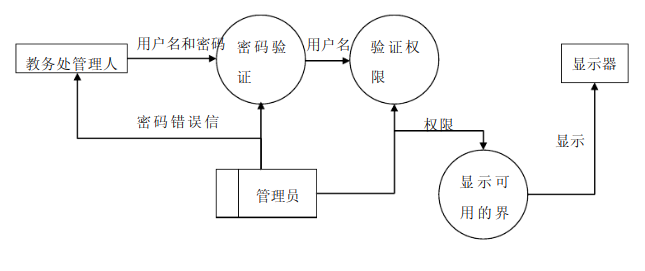
\includegraphics[width=0.7\textwidth]{选区_003} %插入图片,[]中设置图片大小,{}中是图片文件名
    \caption{服务端基本流程} %最终文档中希望显示的图片标题
    \label{Fig.main2} %用于文内引用的标签
\end{figure}

\subsection{基础数据管理}
“基础数据管理”功能模块用于维护整个教务系统正常运行所需的基础数据集,以保证
教务系统有一个统一的标准的基础数据集,便于数据的共享使用,内容包括入学年份、学年学期、院系数据、专业设置等。

\subsection{“学生成绩管理”功能模块}
“学生成绩管理”功能模块用于学生成绩管理系统提供了强大的学生成绩管理管理功能,对学生的各个学期的学生成绩进行保存记录。对学生成绩等信息的添加.修改.删除.查询.汇总.统计等操作。

\subsection{“学籍管理”功能模块}
“学籍管理”主要包括了高校学籍管理的常用信息,提供对学生学籍基本信息录入、查询、修改、打印输出、维护等常用功能,并提供学号编排、学生照片输入与显示、学籍变动(留级、休学、跳级、转班、转学、退学等)、奖惩登记、毕业情况

\subsection{“教室安排”功能模块}
“排课选课管理”功能模块用于根据教学计划、教室资源、教师资源等,制定每学期的课程表。用于对某学期全校课程进行设置,如课表统一制定、每天上课节数、统一的排课时段进行设置。对某个班级某学期具体开设的课程分别进行排课时段、单双周、连常课等特殊情况设置

\subsection{“考务成绩管理”功能模块}
“考务成绩管理”功能模块用于根据课程自动生成本学期的考试地点、考试时间、监考老师等数据,并对考试的过程和结果进行监控。“考务住处发布”用于发布考务信息,如学年、学期、期中(期末)考试、考试时间等,以及其他一些有关考务的事项。 “考试日程安排“用于对评卷专业、评卷科目、评卷教师、评卷日期、时间等评卷信息进行管理。“学生成绩录入”用于授课教师输入学生的考试成绩。(学生学籍信息表)

\subsection{“学生选课”功能模块}
“学生选课”功能模块用于对在校学生个学期的选课情况记录,包括所选课程、教室 安排、选课时间(学期)、选修的课程所在教室、以及对各个选修的课程的成绩记录修改等内容

\section{总体功能结构设计}
\begin{figure}[H] %H为当前位置,!htb为忽略美学标准,htbp为浮动图形
    \centering %图片居中
    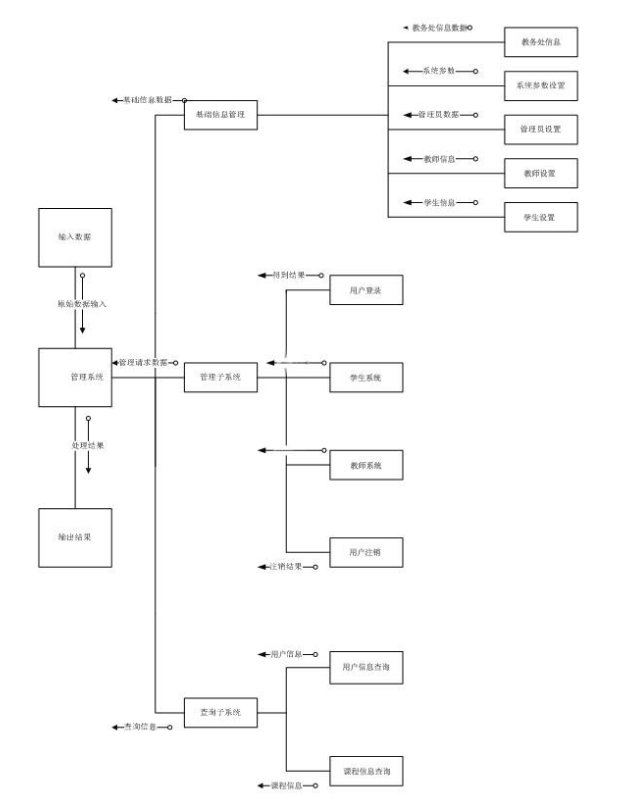
\includegraphics[width=0.7\textwidth]{选区_005} %插入图片,[]中设置图片大小,{}中是图片文件名
    \caption{总体功能结构设计} %最终文档中希望显示的图片标题
    \label{Fig.main2} %用于文内引用的标签
\end{figure}

